\begin{figure}[hbt!]
    \pgfmathsetmacro{\radius}{0.075}
    \pgfmathsetmacro{\sepradius}{4*\radius}
    \pgfmathsetmacro{\inbend}{45}
    \pgfmathsetmacro{\outbend}{180-\inbend}
    \pgfmathsetmacro{\ovalspacing}{0.15}
    \centering
    \begin{subfigure}{\textwidth}
        \centering
        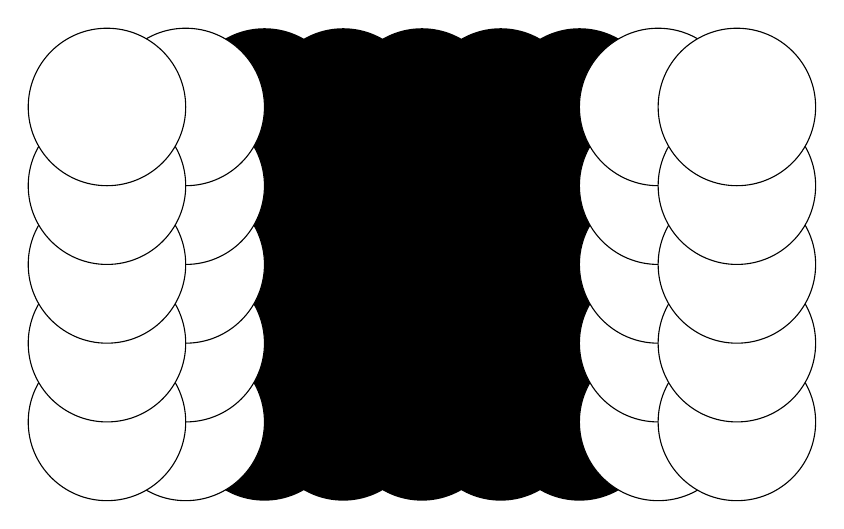
\begin{tikzpicture}
            \draw[very thin, step=1] (0,0) grid(4,4);
            \draw[very thin, dashed,step=1] (-1,0) grid(-2.5,4);
            \draw[very thin, dashed,step=1] (5,0) grid(6.5,4);
            \foreach \x in {0,...,4}{
                \foreach \y in {0,...,4}{
                    \fill (\x,\y) circle(\radius);
                }
            }
            \foreach \x in {-1,-2,5,6}{
                \foreach \y in {0,...,4}{
                    \filldraw[fill=white] (\x,\y) circle(\radius);
                }
            }

        \end{tikzpicture}
        \caption{Normally, one processor only has a local lattice and no data from the neighboring sub-lattices. An empty copy of the sub-lattice is made, to store the shifted lattice.}
    \end{subfigure}
    \begin{subfigure}{\textwidth}
        \centering
        \begin{tikzpicture}
            % Motion
            \draw[very thin, step=1] (0,0) grid(4,4);
            \draw[very thin, dashed,step=1] (-1,0) grid(-2.5,4);
            \draw[very thin, dashed,step=1] (5,0) grid(6.5,4);
            \foreach \x in {0,...,4}{
                \foreach \y in {0,...,4}{
                    \fill (\x,\y) circle(\radius);
                }
            }
            \foreach \x in {-1,-2,5,6}{
                \foreach \y in {0,...,4}{
                    \filldraw[fill=white] (\x,\y) circle(\radius);
                }
            }
            \foreach \x in {0,...,5}{
                \foreach \y in {0,...,4}{
                    \draw (\x,\y) ++(\outbend:\sepradius) coordinate(A);
                    \draw (\x-1,\y) ++(\inbend:\sepradius) coordinate (B);
                    \path[->] (A)  edge[bend right=\inbend] (B);
                }
            }
            \foreach \x in {0,4}{
                \draw (\x-\ovalspacing,-\radius) coordinate (A);
                \draw (A) ++(0,4+2*\radius) coordinate (B);
                \draw (\x+\ovalspacing,-\radius) coordinate (C);
                \draw (C) ++(0,4+2*\radius) coordinate (D);
                \draw[gray] (A) -- (B);
                \draw[gray] (C) -- (D);
                \draw[gray] (A) arc(180:360:\ovalspacing);
                \draw[gray] (D) arc(0:180:\ovalspacing);
            }
        \end{tikzpicture}
        \caption{The shifted lattice is filled with the neighboring links, some of which are received by the ``forward'' neighbor (so some are sent as well to the ``backward'' neighbor)}
        \label{subfig:shift}
    \end{subfigure}
    \begin{subfigure}{\textwidth}
        \centering
        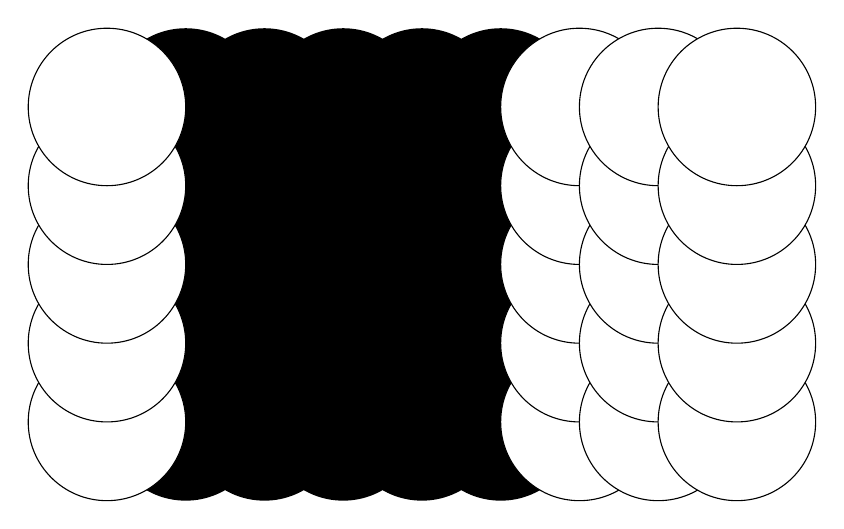
\begin{tikzpicture}
            \draw[very thin, step=1] (0,0) grid(4,4);
            \draw[very thin, dashed,step=1] (-1,0) grid(-2.5,4);
            \draw[very thin, dashed,step=1] (5,0) grid(6.5,4);
            \foreach \x in {-1,...,3}{
                \foreach \y in {0,...,4}{
                    \fill (\x,\y) circle(\radius);
                }
            }
            \foreach \x in {-2,4,5,6}{
                \foreach \y in {0,...,4}{
                    \filldraw[fill=white] (\x,\y) circle(\radius);
                }
            }
        \end{tikzpicture}
        \caption{The shifted lattice is now a local object mapped with the same indices as the original one. A site-by-site multiplication is now possible between the original and the shifted lattices.}
    \end{subfigure}
    \caption{Parallelization scheme based on lattice shifts. When, for example in the staples computation, a link needs to be multiplied by a neighboring one, a new lattice is created. It is filled with the shifted link, which is fetched either from the local sub-lattice if it is in the central region, or from the neighbors if it is on the edge. This schematic drawing shows how a shift along the ``right'' direction is performed. A new lattice containing the data of the target link is created by filling it with the target links. The circled regions in \cref{subfig:shift}, the edges, are shared using MPI by first creating a ``buffer'' of the shape of the edge (it is a cube in the real simulation) and it is sent in a single message to the neighbor which unpacks it in the right location. The new lattice is the multiplied with the original one on a site by site basis, which now is only a local operation.}
    \label{fig:shift}
\end{figure}